\section{Baseline 3}
Terminada a \textit{baseline 2}, o projeto encontra-se exatamente a metade da duração inicialmente prevista, ou seja os tais 51 dias úteis que se referem à data de 10/9/2019, mas o que se encontra concluido até ao momento é apenas metade do previsto, idêntica ou muito semelhante à estabelecida na \textit{baseline 1}, e para isso existem enumeras estratégias possíveis.
\subsection{Estratégia}
Das várias estratégias que tinhamos disponíveis, decidimos optar inicialmente e maioritariamente pela adição de mais recursos, neste caso específico, apenas membros que já se encontravam na equipa mas que não estariam até então atribuidos às atividades que faltavam realizar. Apenas com esta mudança e assumindo neste projeto que, duas pessoas a trabalhar ao mesmo tempo na mesma atividade, irá resultar na redução para metade a duração da mesma (noutros projetos pode não se verificar esta causa-efeito) iremos ter já uma alargada redução relativamente aos tempos, mas mesmo assim não seria suficiente. De modo então a complementar este progresso no tempo restante do projeto, decidimos alterar o método de abordagem numa das fases do mesmo.

A fase previamente referida é na análise da informação, mais especificamente na sub-atividade análise dos risco, e a alteração efetuada foi ao invés de possuirmos simplesmente uma equipa que iria realizar as atividades relativamente a cada instituição seguindo uma relação \textit{finish-to-start}, passamos a ter duas equipas compostas pelos mesmos cargos e de tamanhos idênticos, mas com elementos diferentes, e dividimos de forma equivalente as mesmas. Nesta situação podemos então passar a ter sempre duas instituições a serem analisadas ao mesmo tempo.

\subsection{Resultado}
Realizadas as alterações descritas na estratégia, conseguimos voltar a ter uma previsão de data de finalização de projeto equivalente à calculada na \textit{baseline 1}, que seria dia 21/11/2019 que era o grande objetivo desta \textit{baseline}.
Efetuadas as alterações, e com o acréscimo no uso de recursos, iremos ter também uma desvantagem óbvia que num caso real poderia ser uma entrave à estratégia aqui adotada. Essa desvantagem seria claramente o aumento de custos, que como é demonstrado de seguida, sofrem um aumento considerável.

Nesta fase final do projeto, o mesmo encontra-se concluido a 100\% e por isso, o custo haveria de ser igual ao custo restante mas isso não se verifica, e isso provavelmente deve-se às alterações que foram efetuadas na mesma para conseguir terminar na data prevista. O que era previsível era que o custo aumenta-se uma vez que foi necessário recorrer a mais recursos mas a unica explicação passível nesta situação é que o planeamento das últimas fazes acabou por ficar melhor organizado em termos de custos relativamente ao inicial, pois apesar de mais recursos, são usados em menos quantidade (tempo).

\begin{center}
    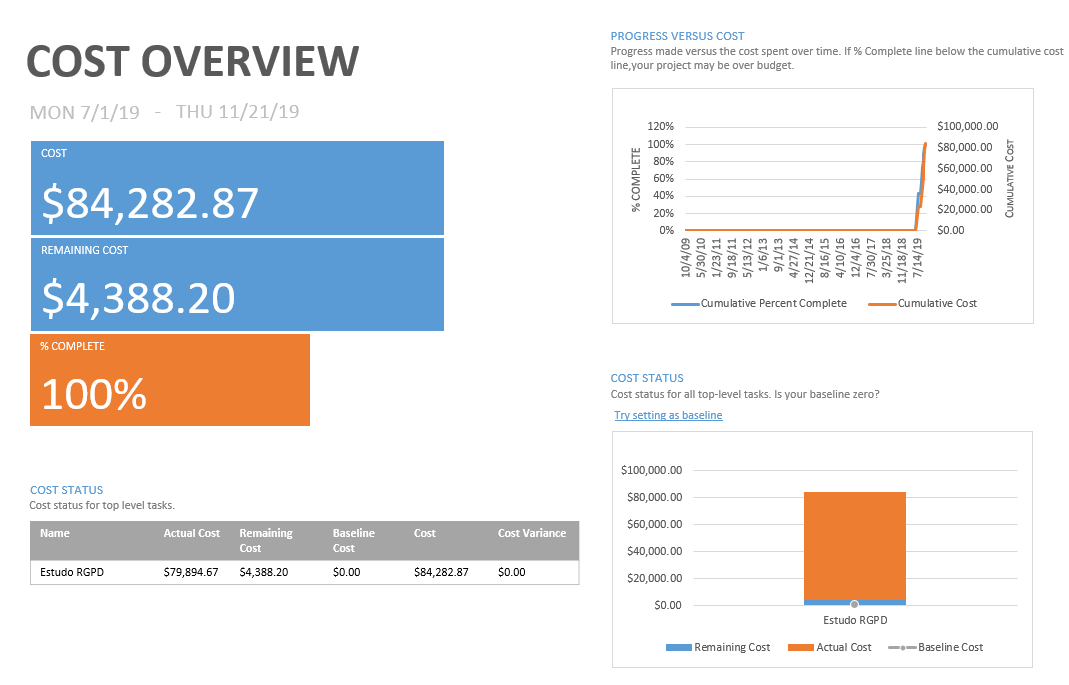
\includegraphics[width=0.7\textwidth]{media/baseline3CostOverview.PNG}
    \captionof{figure}{\textit{Baseline 3} - \textit{Cost Overview}}
\end{center}

\begin{center}
    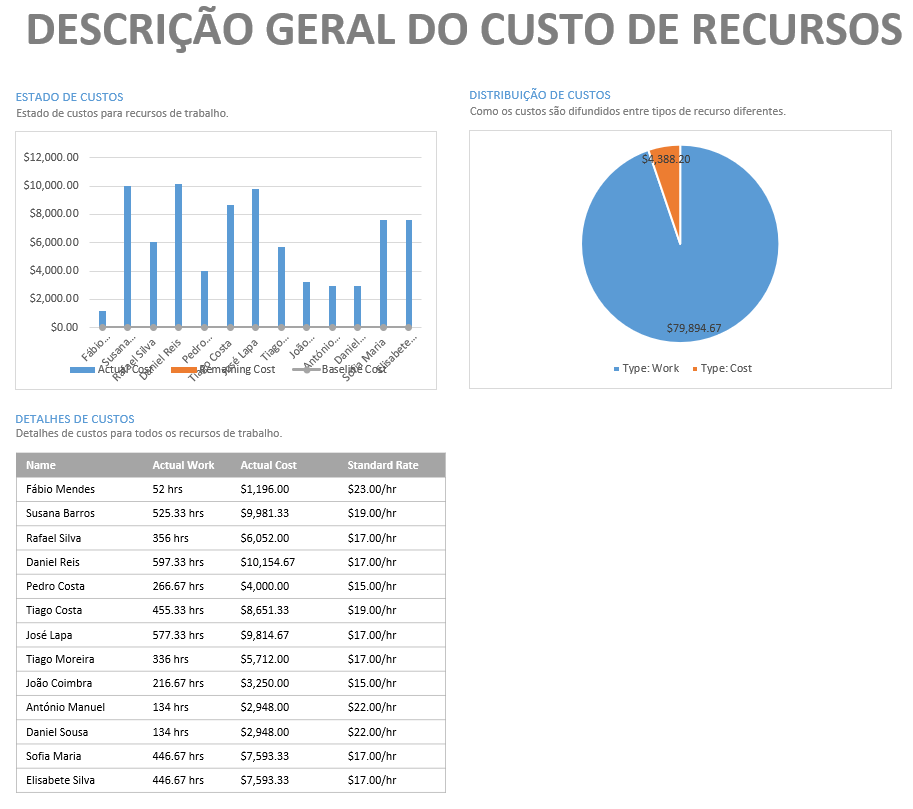
\includegraphics[width=0.7\textwidth]{media/baseline3ResourcesCost.PNG}
    \captionof{figure}{\textit{Baseline 3} - \textit{Resources Cost}}
\end{center}

\begin{center}
    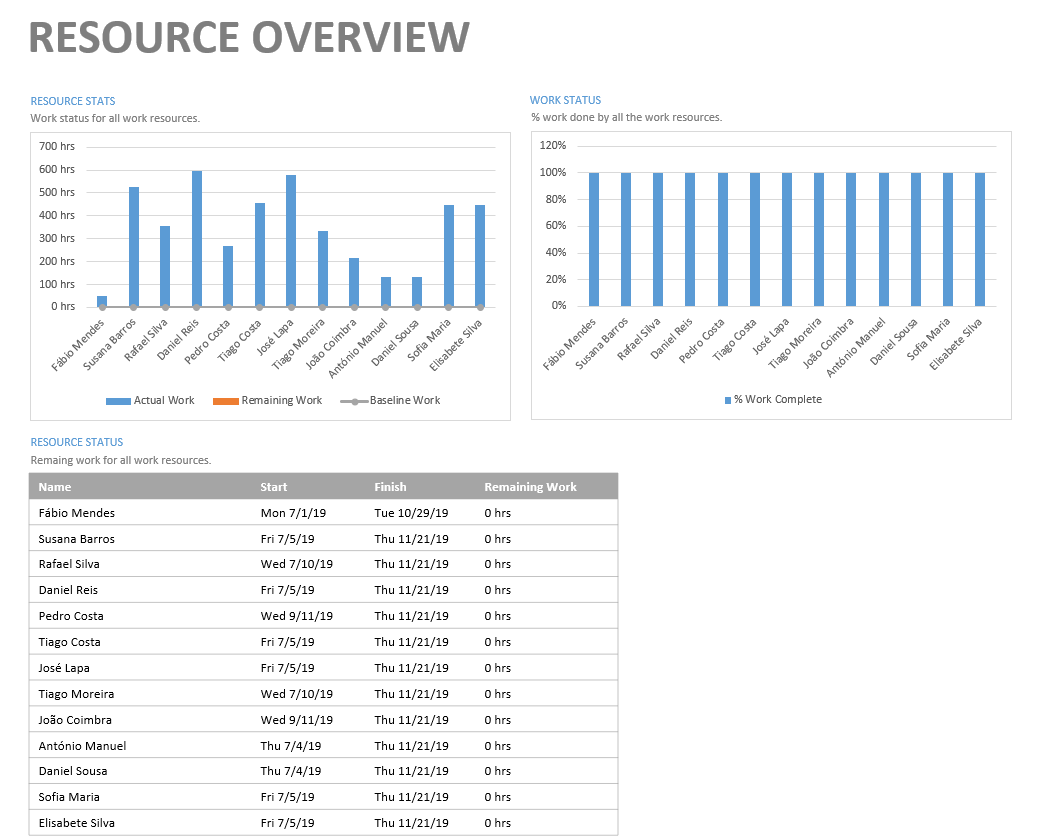
\includegraphics[width=0.7\textwidth]{media/baseline3ResourcesOverview.PNG}
    \captionof{figure}{\textit{Baseline 3} - \textit{Resources Overview}}
\end{center}

Quanto ao \textit{Earned Value} neste caso já irá possuir um valor de acordo com o esperado.

\begin{center}
    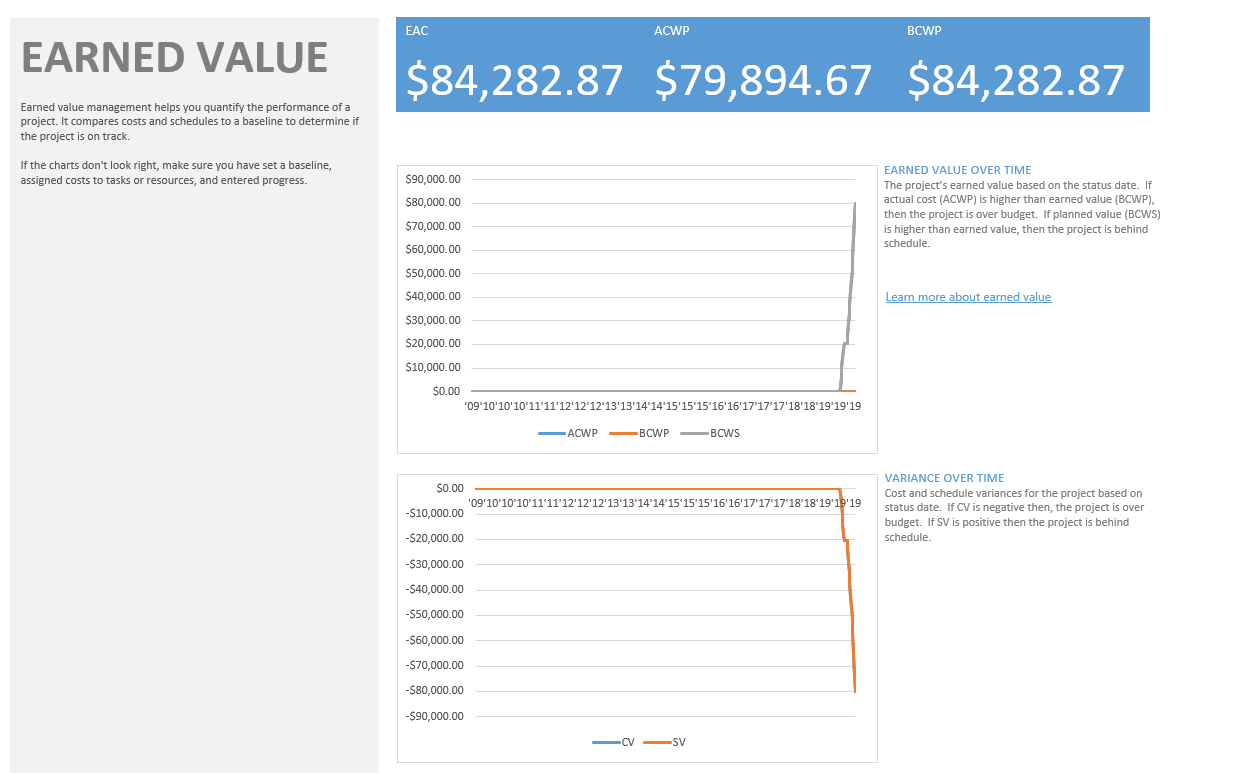
\includegraphics[width=0.7\textwidth]{media/baseline3EarnedValue1.PNG}
    \captionof{figure}{\textit{Baseline 3} - \textit{Earned Value 1}}
\end{center}

\begin{center}
    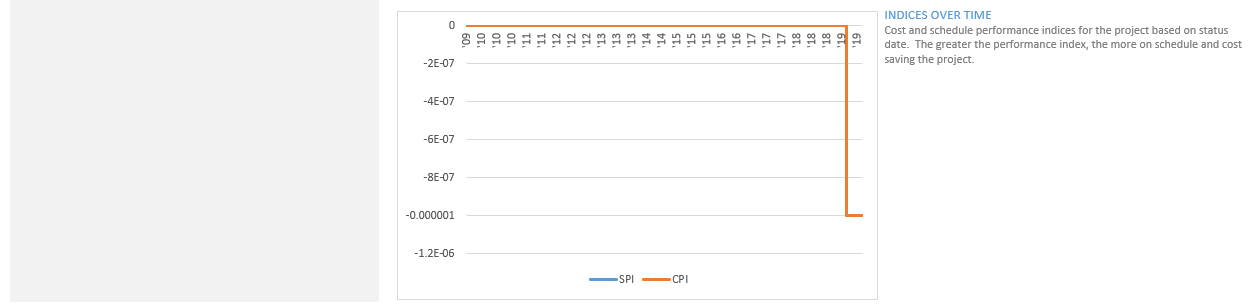
\includegraphics[width=0.7\textwidth]{media/baseline3EarnedValue2.PNG}
    \captionof{figure}{\textit{Baseline 3} - \textit{Earned Value 2}}
\end{center}
